% $Header: /cvsroot/latex-beamer/latex-beamer/solutions/generic-talks/generic-ornate-15min-45min.en.tex,v 1.5 2007/01/28 20:48:23 tantau Exp $

\documentclass{beamer}
%\documentclass[mathsherif]{beamer}

% This file is a solution template for:

% - Giving a talk on some subject.
% - The talk is between 15min and 45min long.
% - Style is ornate.



% Copyright 2004 by Till Tantau <tantau@users.sourceforge.net>.
%
% In principle, this file can be redistributed and/or modified under
% the terms of the GNU Public License, version 2.
%
% However, this file is supposed to be a template to be modified
% for your own needs. For this reason, if you use this file as a
% template and not specifically distribute it as part of a another
% package/program, I grant the extra permission to freely copy and
% modify this file as you see fit and even to delete this copyright
% notice.


\mode<presentation>
{
\usecolortheme[RGB={89,165,140}]{structure}

  \usetheme{Warsaw}
\setbeamercolor*{palette quaternary}{fg=white,bg=structure!40!black}


% o Singapore
% \setbeamercolor{normal text}{bg=blue!10} % para azul, la oscuridad del color se regula cambiando (!20)
% \beamertemplateshadingbackground{yellow!50}{magenta!50} % degradado de amarillo a magenta
  % or ...
% \setbeamertemplate{navigation symbols}{} quitar l\'{\i}nea de s\'{\i}mbolos esquina inferior derecha -in\'{u}tiles
  \setbeamercovered{transparent}
  % or whatever (possibly just delete it)
}


\usepackage[spanish]{babel}
% or whatever

\usepackage[utf8]{inputenc}
% or whatever

\usepackage{times}
\usepackage[T1]{fontenc}
\usepackage{lmodern}

%\usepackage{lucidaso}
%\usepackage[small]{eulervm}

% Paquetes de David
\usepackage{verbatim}
\usepackage{listings}
\usepackage{color}
\usepackage{etoolbox}
\usepackage{xstring}
\usepackage{../gsi-parametros}
 
\definecolor{dkgreen}{rgb}{0,0.6,0}
\definecolor{gray}{rgb}{0.5,0.5,0.5}
\definecolor{mauve}{rgb}{0.58,0,0.82}
  
\lstset{ %
  language=C,                % the language of the code
  basicstyle=\footnotesize,           % the size of the fonts that are used for the code
  %numbers=left,                   % where to put the line-numbers
  numberstyle=\tiny\color{gray},  % the style that is used for the line-numbers
  numbersep=5pt,                  % how far the line-numbers are from the code
%  backgroundcolor=\color{white},      % choose the background color. You must add \usepackage{color}
  showspaces=false,               % show spaces adding particular underscores
  showstringspaces=false,         % underline spaces within strings
  showtabs=false,                 % show tabs within strings adding particular underscores
  %frame=single,                   % adds a frame around the code
  rulecolor=\color{black},        % if not set, the frame-color may be changed on line-breaks within not-black text (e.g. commens (green here))
  tabsize=2,                      % sets default tabsize to 2 spaces
  captionpos=b,                   % sets the caption-position to bottom
  breaklines=true,                % sets automatic line breaking
  breakatwhitespace=false,        % sets if automatic breaks should only happen at whitespace
  %title=\lstname,                   % show the filename of files included with \lstinputlisting;
  keywordstyle=\color{blue},          % keyword style
  commentstyle=\color{dkgreen},       % comment style
  stringstyle=\color{mauve},         % string literal style
  escapeinside={\%*}{*)},            % if you want to add a comment within your code
  morekeywords={*,...}               % if you want to add more keywords to the set
}


% Or whatever. Note that the encoding and the font should match. If T1
% does not look nice, try deleting the line with the fontenc.

% para Singapore
%\setbeamertemplate{footline}{%
%\leavevmode%
%\hbox{%
%\begin{beamercolorbox}[wd=.333333\paperwidth,ht=2.25ex,dp=1ex,center]{author in head/foot}%
%\usebeamerfont{author in head/foot}\insertshortauthor
%\end{beamercolorbox}%
%\begin{beamercolorbox}[wd=.333333\paperwidth,ht=2.25ex,dp=1ex,center]{title in head/foot}%
%\usebeamerfont{title in head/foot}\insertshorttitle
%\end{beamercolorbox}%
%\begin{beamercolorbox}[wd=.333333\paperwidth,ht=2.25ex,dp=1ex,right]{date in head/foot}%
%\usebeamerfont{date in head/foot}\insertshortdate{}\hspace*{2em}
%\insertframenumber{} / \inserttotalframenumber\hspace*{2ex}
%\end{beamercolorbox}}%
%\vskip0pt%
%}
%
% para Warsaw
\newcommand*\oldmacro{}%
\let\oldmacro\insertshorttitle%
\renewcommand*\insertshorttitle{%
  \oldmacro\hfill%
  \insertframenumber\,/\,\inserttotalframenumber}

%\renewcommand*{\appendixname}{Referencias}


\title[Escritura de un texto científico] % (optional, use only with long paper titles)
{Escritura de un texto científico}

\subtitle
{} % (optional)

\author[\asignatura] % (optional, use only with lots of authors)dvanced Robot Control
{\autor}
% - Use the \inst{?} command only if the authors have different
%   affiliation.

\institute[Universidad de Alcal\'{a}] % (optional, but mostly needed)
{
  %\inst{1}%
  \textcolor{structure} {\emph{\textbf{Departamento de Autom\'{a}tica}}}\\
  Universidad de Alcal\'{a}

% - Use the \inst command only if there are several affiliations.
% - Keep it simple, no one is interested in your street address.

%\date[Short Occasion] % (optional)
%{Date / Occasion}

\vspace*{0.5cm}

\includegraphics[height=0.8cm]{comun/uah}
}
\date{}



%logos s\'{o}lo en title
\titlegraphic{
  
\includegraphics[scale=0.45]{comun/dpto}
  \hfill
 % 
\includegraphics[scale=0.35]{gso1}
 % \hfill
  
\includegraphics[scale=0.20]{comun/gso1}
}

% logos tal cual: salen en todos los frames...
%\pgfdeclareimage[height=0.4cm]{left-logo}{gso1}
%\pgfdeclareimage[height=0.4cm]{right-logo}{gso1}
%\logo{\pgfuseimage{right-logo}}


%\setbeamertemplate{sidebar left}
%{
%\logo{\pgfuseimage{left-logo}}
%\vfill%
%\rlap{\hskip0.1cm\insertlogo}%
%\vskip15pt%
%}

\subject{Talks}
% This is only inserted into the PDF information catalog. Can be left
% out.



% If you have a file called "university-logo-filename.xxx", where xxx
% is a graphic format that can be processed by latex or pdflatex,
% resp., then you can add a logo as follows:


% marca de agua de una imagen

\usebackgroundtemplate{
\includegraphics[width=\paperwidth]{comun/marcadeagua}}


%% QUITAR LOS PARES %% DE LAS L\'{I}NEAS DE \AtBeginSubsection PARA QUE SE GENERE LA NAVEGACI\'{O}N EN LA SUBSECCIONES
%%\AtBeginSubsection[]
%% {
%%     \begin{frame}{\'{I}ndice}
%  \small
%  \tableofcontents[currentsection,hideothersubsections]
%  \normalsize
% \end{frame}

%%    \small
%%    \tableofcontents[currentsection,currentsubsection]
     % \tableofcontents[pausesections]
%%   \end{frame}
%%}

%% QUITAR LOS PARES %% DE LAS L\'{I}NEAS DE \AtBeginSubsection PARA QUE SE GENERE LA NAVEGACI\'{O}N EN LA SUBSECCIONES
%%\AtBeginSection[]
%% {
%%     \begin{frame}{\'{I}ndice}
%  \small
%  \tableofcontents[currentsection,hideothersubsections]
%  \normalsize
% \end{frame}

%%    \small
%%    \tableofcontents[currentsection]
     % \tableofcontents[pausesections]
%%   \end{frame}
%%}

% If you wish to uncover everything in a step-wise fashion, uncomment
% the following command:

%\beamerdefaultoverlayspecification{<+->}


\begin{document}

\begin{frame}[plain]
  \titlepage
\end{frame}

\begin{frame}[shrink]{Table of Contents}
 \frametitle{Table of Contents}
 \tableofcontents

 % no me vale: deja descolgado el cap\'{\i}tulo 4
 % \frame[allowframebreaks]%
 %    {\frametitle{\'{I}ndice}\tableofcontents[part=4]}
  % You might wish to add the option [pausesections]
\end{frame}


% Since this a solution template for a generic talk, very little can
% be said about how it should be structured. However, the talk length
% of between 15min and 45min and the theme suggest that you stick to
% the following rules:

% - Exactly two or three sections (other than the summary).
% - At *most* three subsections per section.
% - Talk about 30s to 2min per frame. So there should be between about
%   15 and 30 frames, all told.

\section{Introducción}

\begin{frame}{Introducción}{¿Qué es publicable?}
 	\begin{itemize}
		\item \alert{¿Qué es publicable?}
  			\begin{itemize}
			\item Básicamente, una \alert{contribución}
   			\end{itemize}
		\item Contribución: Aportación al conocimiento
  			\begin{itemize}
			\item Por lo general, una contribución es \alert{algo nuevo}
  				\begin{itemize}
				\item Nueva teoría, nuevo algoritmo, aplicación de un algoritmo conocido a un problema, resolución de un problema original, ...
   				\end{itemize}
			\item Qué se entiende por contribución depende del área
   			\end{itemize}
		\item Casi todo es publicable
  			\begin{itemize}
			\item Es cuestión de cómo presentarlo ...
			\item ... y de dónde publicarlo
   			\end{itemize}
		\item Concepto interesante: ``Contribución mínima publicable''
   	\end{itemize}
\end{frame}

\section{Estructura de un artículo}
\subsection{Estructura básica}

\begin{frame}{Estructura de un artículo} {Estructura básica}
	\begin{block}{Estructura}
	\begin{columns}
		\column{.5\textwidth}
			\begin{itemize}
				\item Título
				\item Autores y afiliación
				\item Resumen (\textit{abstract})
				\item Palabras clave
			\end{itemize}

		\column{.5\textwidth}
			\begin{itemize}
				\item Introducción
				\item Marco teórico
				\item Trabajo relacionado
				\item Núcleo del artículo
				\item Experimentación
				\item Conclusiones
				\item Agradecimientos
				\item Bibliografía
			\end{itemize}
		\end{columns}
	\end{block}
\end{frame}

\subsection{Partes de un artículo}
\begin{frame}{Estructura de un artículo} {Partes de un artículo: Título}
	\begin{columns}
	\column{.45\textwidth}
	\begin{itemize}
		\item Reflejar contenido
			\begin{itemize}
			\item Corto, preciso e informativo
			\item Gramaticalmente correcto
			\end{itemize}
		\item A evitar:
			\begin{itemize}
			\item Título largo
			\item Ambigüedad
			\item Terminar con punto
			\end{itemize}
		\item Se busca:
			\begin{itemize}
			\item \alert{Brevedad y precisión}
			\item Captar atención
			\item Título ``sexy''
			\end{itemize}
	\end{itemize}

	\column{.6\textwidth}
	\begin{block}{Malos ejemplos}
  	\begin{center}
	\textit{``In the end, there can be only ones''}\\
	\textit{``The One-Max Algorithm. Evolutionary Computing''}
	\end{center}
	\end{block}

	\begin{block}{Buenos ejemplos}
  	\begin{center}
	\textit{``Allocating educational resources through happiness maximization''}\\
	\textit{``A Multi-Agent Simulation Platform Applied to the Study of Urban Traffic Lights ''}
	\end{center}
	\end{block}
	\end{columns}
\end{frame}

\begin{frame}{Estructura de un artículo} {Partes de un artículo: Autores y afiliación (I)}
	\begin{itemize}
		\item Incluir a quienes hayan hecho contribución substancial
			\begin{itemize}
			\item Tema políticamente delicado
			\begin{itemize}
			\item A veces, mucha gente contribuye
			\item Otras (las más), mucha gente quiere aparecer
			\end{itemize}
			\item Sugerencia: Reglas objetivas a nivel de grupo
			\end{itemize}
		\item El orden de los factores altera el producto
			\begin{itemize}
			\item No es igual ser primer autor que último
			\item Vuelve a ser un tema delicado
			\item Sugerencia: Reglas objetivas a nivel de grupo
			\end{itemize}
		\item Poner nombre completo, sin iniciales
			\begin{itemize}
			\item Bueno: David F. Barrero o David Fernández Barrero
			\item Malo: D. F. Barrero
			\end{itemize}
		\item Incorporar, al menos, correo electrónico
	\end{itemize}
\end{frame}

\begin{frame}{Estructura de un artículo} {Partes de un artículo: Autores y afiliación (II)}
	\begin{itemize}
		\item \alert{Corresponding author}: Enlaza al resto de autores
			\begin{itemize}
			\item Normalmente, el primer autor
			\end{itemize}
		\item IMPORTANTE: Usar siempre el mismo nombre
			\begin{itemize}
			\item Más fácil para indexadores
			\item Facilita ver impactos y cálculo de H
			\end{itemize}
	\end{itemize}
	\begin{columns}
	\column{.6\textwidth}
	\begin{block}{Consejos}
		\centering Usar el apellido menos común\\
		\centering Juntar apellidos con guión
	\end{block}
	\end{columns}
\end{frame}

\begin{frame}{Estructura de un artículo} {Partes de un artículo: Resumen (I)}
	\begin{itemize}
		\item Texto de unas \alert{200 palabras}
		\item Tiene que resumir el trabajo y \alert{captar la atención}
		\begin{itemize}
		\item Propósito de la investigación
		\item Descripción de la teoría o experimentación realizada
		\item Resumen de contribuciones
		\item Mencionar principales conclusiones
		\end{itemize}
		\item Debe ser autocontenido
	\end{itemize}
\end{frame}

\begin{frame}{Estructura de un artículo} {Partes de un artículo: Resumen (II)}
	Una posible estructura de resumen:
		\begin{enumerate}
		\item Introducir el problema
		\item Justificar el interés del problema
		\item Introducir la solución propuesta
		\item Justificar el interés de la solución propuesta
		\item Principales conclusiones
		\end{enumerate}
	Recuerden, ¡200 palabras!
\end{frame}

\begin{frame}{Estructura de un artículo} {Partes de un artículo: Palabras clave}
	\begin{itemize}
		\item Es opcional
		\item Unas 3-5 palabras relevantes
		\begin{itemize}
			\item A veces la publicación da una lista de palabras clave
		\end{itemize}
		\item Utilidades:
		\begin{itemize}
		\item Identificar temas sin leer el artículo
		\item Facilita búsquedas
		\item Facilita encontrar revisores adecuados
		\end{itemize}
		\item Posiblemente obsoleto en breve ... pero se sigue pidiendo
	\end{itemize}
\end{frame}

\begin{frame}{Estructura de un artículo} {Partes de un artículo: Introducción}
	\begin{itemize}
		\item La introducción ``introduce'' el trabajo
		\begin{itemize}
			\item Objetivos de la investigación
			\item \textit{Contribuciones del artículo}
			\item Precedentes de la literatura
			\item Esbozo de conclusiones
			\item Estructura del artículo
		\end{itemize}
		\item El lector la lee para decidir si seguir leyendo
		\item Una introducción no es:
		\begin{itemize}
			\item Una discución en profundidad (literatura o resultados)
			\item Un adelanto de las conclusiones
			\item Relleno sin contenido
		\end{itemize}
		\item Media página (congreso) o una página (revista)
	\end{itemize}
\end{frame}

\begin{frame}{Estructura de un artículo} {Partes de un artículo: Marco teórico}
	\begin{itemize}
		\item Resumen de la base teórica del trabajo
		\item Contiene la información necesaria para leer el artículo
			\begin{itemize}
			\item El concepto ``base'' depende de la publicación
			\item Introduce las definiciones necesarias
			\item Descripción del problema
			\end{itemize}
		\item No se explican cosas básicas, según publicación
			\begin{itemize}
			\item ¿Qué perfil tiene la publicación?
			\end{itemize}
		\item A veces se fusiona con el trabajo relacionado
	\end{itemize}
\end{frame}

\begin{frame}{Estructura de un artículo} {Partes de un artículo: Trabajo relacionado}
	\begin{itemize}
		\item Revisión de la literatura relacionada
			\begin{itemize}
			\item ¿Qué se ha hecho recientemente que esté relacionado?
			\end{itemize}
		\item Importante: \alert{Referencias actualizadas}
	\end{itemize}
	\begin{columns}
	\column{.7\textwidth}
		\begin{block}{Técnicas de búsqueda}
			\centering Observar las referencias de los artículos\\
			Identificar autores principales\\
			Partir de un artículo de revisión\\
			Buscar qué artículos citan uno dado
		\end{block}
	\end{columns}
\end{frame}

\begin{frame}{Estructura de un artículo} {Partes de un artículo: Núcleo del artículo}
		Presenta la idea central
		\begin{itemize}
			\item Algoritmo, arquitectura, protocolo, teoría, desarrollo formal, ...
		\end{itemize}
	\begin{columns}
	\column{.5\textwidth}
		\begin{block}{Algoritmo}
		\begin{itemize}
			\item Usar pseudocódigo
			\item No dar código
			\item No usar diagramas flujo
		\end{itemize}
		\end{block}

	\column{.5\textwidth}
		\begin{block}{Arquitectura}
		\begin{itemize}
			\item Diagrama arquitectónico
			\item Nivel de subsistema
			\item No descender a código/clase
		\end{itemize}
		\end{block}
	\end{columns}

	\begin{columns}
	\column{.5\textwidth}
	\begin{block}{Teoría}
	\begin{itemize}
		\item Estructura formal
		\item Teorema - demostración
	\end{itemize}
	\end{block}
	\end{columns}	
\end{frame}

\begin{frame}{Estructura de un artículo} {Partes de un artículo: Experimentación}
	\centering Trabajos teóricos pueden no tener experimentación
	\begin{enumerate}
	\item Describir el experimento
		\begin{itemize}
		\item Facilitar la \alert{repetitividad} y \alert{reproducibilidad}
		\item Utilizar pasado simple, evitar pasivo
		\item \alert{Aporta información sobre la pregunta de investigación}
		\end{itemize}
	\item Presentar resultados
		\begin{itemize}
		\item Tablas, gráficos, análisis estadístico
		\end{itemize}
	\item Análisis de los resultados
		\begin{itemize}
		\item Interpretación de los resultados
		\item Opcional: Análisis estadístico
		\end{itemize}
	\end{enumerate}
\end{frame}

\begin{frame}{Estructura de un artículo} {Partes de un artículo: Discusión}
	Opcional: Sección de discusión
		\begin{itemize}
		\item Análisis \textit{en profundidad} de los resultados
		\item Da un paso más allá del dato: Perspectiva amplia
		\item A veces, en tono especulativo
			\begin{itemize}
			\item Especular sobre explicaciones o consecuencias
			\end{itemize}
		\end{itemize}
\end{frame}


\begin{frame}{Estructura de un artículo} {Partes de un artículo: Conclusiones}
	\begin{itemize}
		\item Principales logros del artículo
			\begin{itemize}
			\item ¿Qué debería recordar el lector?
			\end{itemize}
		\item Es un resumen de cosas ya presentadas
			\begin{itemize}
			\item No se presentan resultados nuevos
			\item No se presentan ideas nuevas
			\end{itemize}
		\item Habitualmente se incluye trabajo futuro
			\begin{itemize}
			\item Truco: Convertir debilidades en fortalezas
			\end{itemize}
	\end{itemize}
\end{frame}

\begin{frame}{Estructura de un artículo} {Partes de un artículo: Agradecimientos}
	Dos usos habituales
	\begin{itemize}
		\item Agradecer a personas que aportaron algo al artículo
		\item Incorporar instituciones financiadoras
	\end{itemize}
	\begin{columns}
	\column{.9\textwidth}
	\begin{block}{Ejemplo real}
	\footnotesize{
The authors would like to thank Dr. Bonifacio Castaño Martín and Dr. Concepción Alonso Rodríguez for their valuable suggestions and Mike de Pumpo for proof reading this article. This work has been funded by the Spanish Ministry of Science and Technology under the projects ABANT (TIN2010 19872), Castilla-La Mancha project (PEII11-0079-8929), and by Jobssy.com (FUAM-076913).}
	\end{block}
	\end{columns}
\end{frame}

\begin{frame}{Estructura de un artículo} {Partes de un artículo: Bibliografía}
	\begin{columns}
	\column{.7\textwidth}
	\begin{itemize}
		\item Aunque no lo parezca, es muy importante
		\begin{itemize}
			\item Referencias actualizadas
			\item Referencias completas
			\item Citar a la propia revista/congreso
		\end{itemize}
		\item Limitar las autorreferencias (2-3)
		\item Gestionar referencias es muy complejo
			\begin{itemize}
			\item Afortunadamente, existe {\rm B\kern-.05em{\sc i\kern-.025em b}\kern-.08em
			    T\kern-.1667em\lower.7ex\hbox{E}\kern-.125emX}
			\end{itemize}
		\item \alert{Mantener una base de datos bibliográfica}
			\begin{itemize}
			\item Mantiene resúmenes, comentarios, etc
			\item Imprescindible tener una
			\end{itemize}
	\end{itemize}
	\column{.25\textwidth}
		\begin{block}{Herramientas}
		Mendeley\\
		JabRef\\
		EndNotes
		\end{block}
	\end{columns}
\end{frame}

\section{Cuestiones generales}
\subsection{Generalidades}
\begin{frame}{Cuestiones generales} {Generalidades}
	\begin{itemize}
		\item Un artículo es un \textit{documento formal}
			\begin{itemize}
			\item Usar lenguaje formal
			\item Extremar cuidado con faltas de ortografía
			\end{itemize}
		\item Lenguaje preciso
			\begin{itemize}
			\item Evitar ambigüedades
			\item Usar la palabra precisa para el concepto preciso
			\end{itemize}
		\item Cuidar la redacción
			\begin{itemize}
			\item Frases enlazadas
			\item Definir acrónimo la primera vez que se use
			\end{itemize}
		\item Transiciones suaves entre secciones
			\begin{itemize}
			\item Introducir un pequeño resumen y conclusiones de la sección
			\item Terminar sección dando paso a la siguiente
			\end{itemize}
		\item \alert{Cuidar el inglés}
	\end{itemize}
\end{frame}

\subsection{Gráficos}
\begin{frame}{Cuestiones generales} {Gráficos (I)}
	\begin{itemize}
		\item Útiles para presentar información \textit{visualmente}
		\item Deben facilitar la comprensión de los datos mostrados
		\item Utilizar el gráfico adecuado para el propósito buscado
			\begin{itemize}
			\item \url{http://extremepresentation.typepad.com/.a/6a00d8341bfd2e53ef00e553577fea8833-pi?goback=\%2Egde\_152247\_member\_137236550}
			\item \url{http://labs.juiceanalytics.com/chartchooser.html}
			\end{itemize}
		\item Que sea legible
			\begin{itemize}
			\item Tamaño de letra suficiente
			\item Evitar aglomeraciones
			\item Verificar si se ve en B/N
			\end{itemize}
		\item Indicar unidades
	\end{itemize}
\end{frame}

\begin{frame}[plain]{Cuestiones generales} {Gráficos (II)}
\begin{figure}[t]
 \caption{Maximum expected relative estimation error of $E$ as function of $\mu$, $\sigma$ and $n$, as modeled by (5). The number of runs takes values $n\in\{30,50,100,500\}$, CIs were computed with $\alpha=0.05$ and $E$ with $\varepsilon=0.05$. The SR is, in all the cases, $0.5$.}\label{fig:E-error}\end{figure}
 \vspace{-1.2cm}
\begin{center}
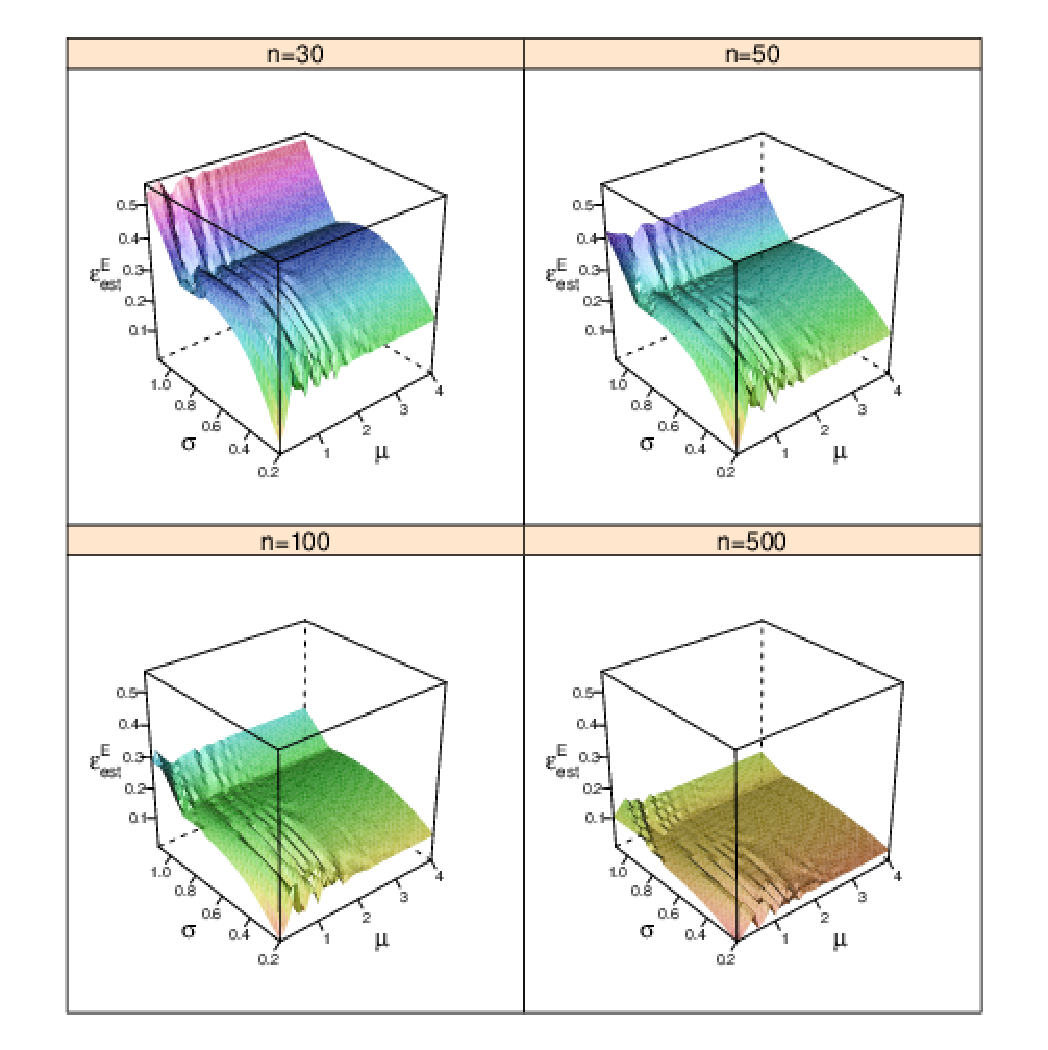
\includegraphics[width=0.6\textwidth]{figs/E-error.pdf}
 \end{center}
\end{frame}

\subsection{Tablas}
\begin{frame}{Cuestiones generales} {Tablas (I)}
	\begin{itemize}
		\item Aportan información tabular
			\begin{itemize}
			\item Importa el número exacto (parámetros de un algoritmo, por ejemplo)
			\item Resúmenes
			\end{itemize}
		\item Usar cuando no se puede sustituir por un gráfico
			\begin{itemize}
			\item Para ``visualizar'' datos, mejor los gráficos
			\end{itemize}
		\item Indicar las unidades
		\item El formato depende de la publicación
	\end{itemize}
\end{frame}

\begin{frame}{Cuestiones generales} {Tablas (II)}
	\footnotesize{\begin{table}[t]
	\begin{center}
	\renewcommand{\arraystretch}{1.3}
	\caption{Estimations of the parameters of the lognormal and shifted exponential for the six problem instances under study. The lognormal distribution has two parameters, the mean $\mu$ and the standard deviation $\sigma$, and the shifted exponential has two parameters, $\lambda$ and the shift $t_0$.\label{tab:exponential}}
	\begin{tabular}{lllllll}
	\hline\noalign{\smallskip}
      & $\hat{\mu}$   & $\hat{\sigma}$ &  $\hat{\lambda}$ & $t_0$ \\
	\noalign{\smallskip} 
	\hline 
	\noalign{\smallskip}
	Artificial ant  & 2.73  & 0.595 & 0.085  & 9    \\ 
	Regression      & 2.289 & 0.44  & 0.150  & 5    \\ 
	4-Parity        & 3.03  & 0.284 & 0.146  & 17   \\ 
	5-Parity        & 5.004 & 0.8   & 0.005  & 7    \\ 
	6-Multiplexer   & 2.464 & 0.425 & 0.149  & 7    \\ 
	11-Multiplexer  & 5.367 & 0.797 & 0.004  & 60   \\ 
	\hline
	\end{tabular}
	\end{center}
	\end{table}}
\end{frame}

\subsection{Fórmulas}
\begin{frame}{Cuestiones generales} {Fórmulas}
	\begin{itemize}
		\item Ayudan a explicar conceptos
			\begin{itemize}
			\item Más formal
			\item Menos espacio
			\item Evita ambigüedad
			\end{itemize}
		\item No usarlas para aparentar seriedad
			\begin{itemize}
			\item ¡Los revisores miran las fórmulas!
			\end{itemize}
		\item Se asocian a un número
			\begin{equation}
			p_{s,i,i-1, ..., 0} = \left[1-(1-p^{(k)'})^M\right] \; \prod_{j=0}^{i-2} \left(1-p^{(k)'}\right)^M%P(S_s=s | S_i=i, S_{i-1}=i-1, ..., S_1=1) = \left[1-(1-p^{(k)'})^M\right] \; \prod_{j=1}^{i-1} \left(1-p^{(k)'}\right)^M
			\end{equation}
			Se referencia el número, por ejemplo, (1)
	\end{itemize}
\end{frame}

\subsection{Otras cuestiones}
\begin{frame}{Cuestiones generales} {Otras cuestiones}
	\begin{itemize}
		\item Figuras y tablas \alert{nunca} se insertan en el texto
			\begin{itemize}
			\item Se identifican por número: Ver Tabla 1; según Figura 4, ...
			\item Poner (y referenciar) en orden consecutivo
			\item Referenciar \alert{todas} las tablas y figuras
			\end{itemize}
			\item Cuestiones sobre redacción
			\begin{itemize}
			\item Definir abreviaciones en su primer uso
			\item Evitar vocabulario no estándar
			\item Utilizar el corrector ortográfico
			\end{itemize}
	\end{itemize}
\end{frame}

\section{Otras cuestiones}
\begin{frame}{Otras cuestiones}{Enlaces útiles}
	\begin{block}{Redes sociales}
	Linkedin: \url{http://www.linkedin.com/}\\
	Mendeley: \url{http://www.mendeley.com/}\\
	Research gate: \url{http://www.researchgate.com/}\\
	I am researcher: \url{http://www.iamresearcher.com/}\\
	Twitter: \url{http://www.twitter.com/}
	\end{block}
	\begin{block}{Otros}
	Feedly: \url{http://feedly.com/}
	\end{block}
\end{frame}



\end{document}
